% Created by tikzDevice version 0.10.1 on 2018-03-11 19:45:45
% !TEX encoding = UTF-8 Unicode
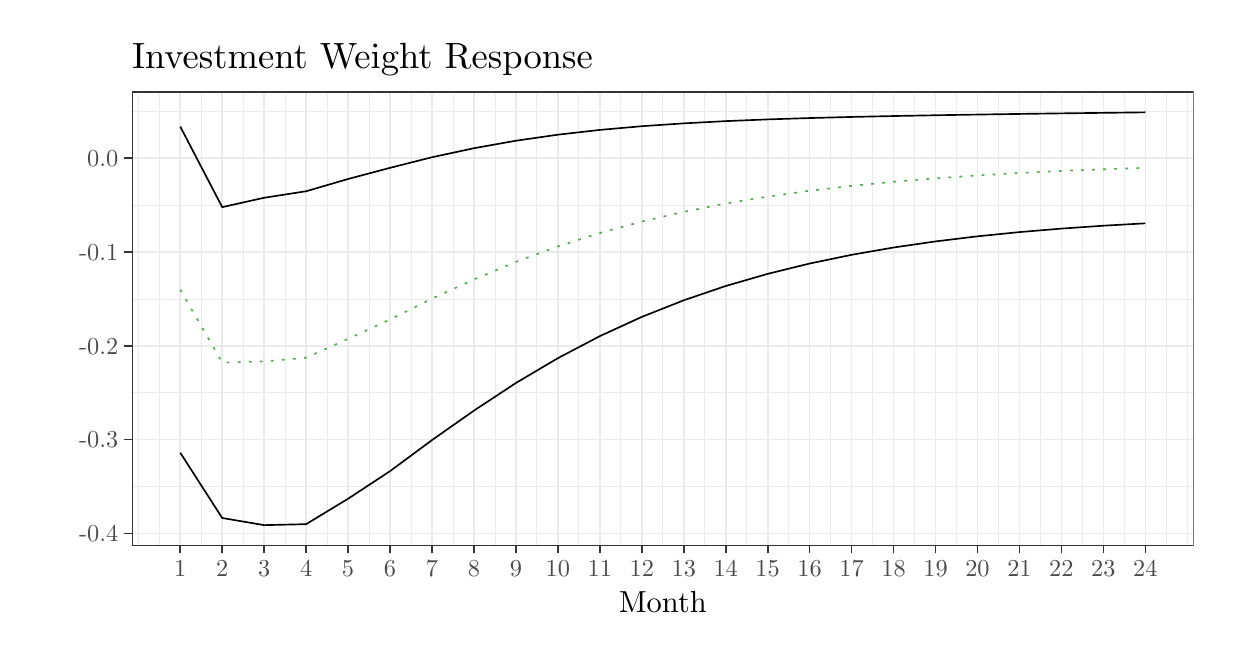
\begin{tikzpicture}[x=1pt,y=1pt]
\definecolor{fillColor}{RGB}{255,255,255}
\path[use as bounding box,fill=fillColor,fill opacity=0.00] (0,0) rectangle (426.79,216.81);
\begin{scope}
\path[clip] (  0.00,  0.00) rectangle (426.79,216.81);
\definecolor{drawColor}{RGB}{255,255,255}
\definecolor{fillColor}{RGB}{255,255,255}

\path[draw=drawColor,line width= 0.6pt,line join=round,line cap=round,fill=fillColor] (  0.00,  0.00) rectangle (426.79,216.81);
\end{scope}
\begin{scope}
\path[clip] ( 37.70, 29.59) rectangle (421.29,193.67);
\definecolor{fillColor}{RGB}{255,255,255}

\path[fill=fillColor] ( 37.70, 29.59) rectangle (421.29,193.67);
\definecolor{drawColor}{gray}{0.92}

\path[draw=drawColor,line width= 0.3pt,line join=round] ( 37.70, 51.01) --
	(421.29, 51.01);

\path[draw=drawColor,line width= 0.3pt,line join=round] ( 37.70, 84.90) --
	(421.29, 84.90);

\path[draw=drawColor,line width= 0.3pt,line join=round] ( 37.70,118.79) --
	(421.29,118.79);

\path[draw=drawColor,line width= 0.3pt,line join=round] ( 37.70,152.68) --
	(421.29,152.68);

\path[draw=drawColor,line width= 0.3pt,line join=round] ( 37.70,186.58) --
	(421.29,186.58);

\path[draw=drawColor,line width= 0.3pt,line join=round] ( 39.97, 29.59) --
	( 39.97,193.67);

\path[draw=drawColor,line width= 0.3pt,line join=round] ( 47.56, 29.59) --
	( 47.56,193.67);

\path[draw=drawColor,line width= 0.3pt,line join=round] ( 62.72, 29.59) --
	( 62.72,193.67);

\path[draw=drawColor,line width= 0.3pt,line join=round] ( 77.88, 29.59) --
	( 77.88,193.67);

\path[draw=drawColor,line width= 0.3pt,line join=round] ( 93.04, 29.59) --
	( 93.04,193.67);

\path[draw=drawColor,line width= 0.3pt,line join=round] (108.20, 29.59) --
	(108.20,193.67);

\path[draw=drawColor,line width= 0.3pt,line join=round] (123.36, 29.59) --
	(123.36,193.67);

\path[draw=drawColor,line width= 0.3pt,line join=round] (138.53, 29.59) --
	(138.53,193.67);

\path[draw=drawColor,line width= 0.3pt,line join=round] (153.69, 29.59) --
	(153.69,193.67);

\path[draw=drawColor,line width= 0.3pt,line join=round] (168.85, 29.59) --
	(168.85,193.67);

\path[draw=drawColor,line width= 0.3pt,line join=round] (184.01, 29.59) --
	(184.01,193.67);

\path[draw=drawColor,line width= 0.3pt,line join=round] (199.17, 29.59) --
	(199.17,193.67);

\path[draw=drawColor,line width= 0.3pt,line join=round] (214.33, 29.59) --
	(214.33,193.67);

\path[draw=drawColor,line width= 0.3pt,line join=round] (229.50, 29.59) --
	(229.50,193.67);

\path[draw=drawColor,line width= 0.3pt,line join=round] (244.66, 29.59) --
	(244.66,193.67);

\path[draw=drawColor,line width= 0.3pt,line join=round] (259.82, 29.59) --
	(259.82,193.67);

\path[draw=drawColor,line width= 0.3pt,line join=round] (274.98, 29.59) --
	(274.98,193.67);

\path[draw=drawColor,line width= 0.3pt,line join=round] (290.14, 29.59) --
	(290.14,193.67);

\path[draw=drawColor,line width= 0.3pt,line join=round] (305.30, 29.59) --
	(305.30,193.67);

\path[draw=drawColor,line width= 0.3pt,line join=round] (320.47, 29.59) --
	(320.47,193.67);

\path[draw=drawColor,line width= 0.3pt,line join=round] (335.63, 29.59) --
	(335.63,193.67);

\path[draw=drawColor,line width= 0.3pt,line join=round] (350.79, 29.59) --
	(350.79,193.67);

\path[draw=drawColor,line width= 0.3pt,line join=round] (365.95, 29.59) --
	(365.95,193.67);

\path[draw=drawColor,line width= 0.3pt,line join=round] (381.11, 29.59) --
	(381.11,193.67);

\path[draw=drawColor,line width= 0.3pt,line join=round] (396.27, 29.59) --
	(396.27,193.67);

\path[draw=drawColor,line width= 0.3pt,line join=round] (411.44, 29.59) --
	(411.44,193.67);

\path[draw=drawColor,line width= 0.3pt,line join=round] (419.02, 29.59) --
	(419.02,193.67);

\path[draw=drawColor,line width= 0.6pt,line join=round] ( 37.70, 34.07) --
	(421.29, 34.07);

\path[draw=drawColor,line width= 0.6pt,line join=round] ( 37.70, 67.96) --
	(421.29, 67.96);

\path[draw=drawColor,line width= 0.6pt,line join=round] ( 37.70,101.85) --
	(421.29,101.85);

\path[draw=drawColor,line width= 0.6pt,line join=round] ( 37.70,135.74) --
	(421.29,135.74);

\path[draw=drawColor,line width= 0.6pt,line join=round] ( 37.70,169.63) --
	(421.29,169.63);

\path[draw=drawColor,line width= 0.6pt,line join=round] ( 55.14, 29.59) --
	( 55.14,193.67);

\path[draw=drawColor,line width= 0.6pt,line join=round] ( 70.30, 29.59) --
	( 70.30,193.67);

\path[draw=drawColor,line width= 0.6pt,line join=round] ( 85.46, 29.59) --
	( 85.46,193.67);

\path[draw=drawColor,line width= 0.6pt,line join=round] (100.62, 29.59) --
	(100.62,193.67);

\path[draw=drawColor,line width= 0.6pt,line join=round] (115.78, 29.59) --
	(115.78,193.67);

\path[draw=drawColor,line width= 0.6pt,line join=round] (130.94, 29.59) --
	(130.94,193.67);

\path[draw=drawColor,line width= 0.6pt,line join=round] (146.11, 29.59) --
	(146.11,193.67);

\path[draw=drawColor,line width= 0.6pt,line join=round] (161.27, 29.59) --
	(161.27,193.67);

\path[draw=drawColor,line width= 0.6pt,line join=round] (176.43, 29.59) --
	(176.43,193.67);

\path[draw=drawColor,line width= 0.6pt,line join=round] (191.59, 29.59) --
	(191.59,193.67);

\path[draw=drawColor,line width= 0.6pt,line join=round] (206.75, 29.59) --
	(206.75,193.67);

\path[draw=drawColor,line width= 0.6pt,line join=round] (221.91, 29.59) --
	(221.91,193.67);

\path[draw=drawColor,line width= 0.6pt,line join=round] (237.08, 29.59) --
	(237.08,193.67);

\path[draw=drawColor,line width= 0.6pt,line join=round] (252.24, 29.59) --
	(252.24,193.67);

\path[draw=drawColor,line width= 0.6pt,line join=round] (267.40, 29.59) --
	(267.40,193.67);

\path[draw=drawColor,line width= 0.6pt,line join=round] (282.56, 29.59) --
	(282.56,193.67);

\path[draw=drawColor,line width= 0.6pt,line join=round] (297.72, 29.59) --
	(297.72,193.67);

\path[draw=drawColor,line width= 0.6pt,line join=round] (312.89, 29.59) --
	(312.89,193.67);

\path[draw=drawColor,line width= 0.6pt,line join=round] (328.05, 29.59) --
	(328.05,193.67);

\path[draw=drawColor,line width= 0.6pt,line join=round] (343.21, 29.59) --
	(343.21,193.67);

\path[draw=drawColor,line width= 0.6pt,line join=round] (358.37, 29.59) --
	(358.37,193.67);

\path[draw=drawColor,line width= 0.6pt,line join=round] (373.53, 29.59) --
	(373.53,193.67);

\path[draw=drawColor,line width= 0.6pt,line join=round] (388.69, 29.59) --
	(388.69,193.67);

\path[draw=drawColor,line width= 0.6pt,line join=round] (403.86, 29.59) --
	(403.86,193.67);
\definecolor{drawColor}{RGB}{77,175,74}

\path[draw=drawColor,line width= 0.6pt,dash pattern=on 1pt off 3pt ,line join=round] ( 55.14,122.13) --
	( 70.30, 95.80) --
	( 85.46, 96.20) --
	(100.62, 97.55) --
	(115.78,104.36) --
	(130.94,111.36) --
	(146.11,118.89) --
	(161.27,125.84) --
	(176.43,132.19) --
	(191.59,137.76) --
	(206.75,142.60) --
	(221.91,146.74) --
	(237.08,150.27) --
	(252.24,153.25) --
	(267.40,155.76) --
	(282.56,157.87) --
	(297.72,159.64) --
	(312.89,161.12) --
	(328.05,162.37) --
	(343.21,163.41) --
	(358.37,164.29) --
	(373.53,165.02) --
	(388.69,165.64) --
	(403.86,166.16);
\definecolor{drawColor}{RGB}{0,0,0}

\path[draw=drawColor,line width= 0.6pt,line join=round] ( 55.14, 63.21) --
	( 70.30, 39.63) --
	( 85.46, 37.05) --
	(100.62, 37.40) --
	(115.78, 46.59) --
	(130.94, 56.56) --
	(146.11, 67.79) --
	(161.27, 78.43) --
	(176.43, 88.42) --
	(191.59, 97.38) --
	(206.75,105.35) --
	(221.91,112.29) --
	(237.08,118.30) --
	(252.24,123.46) --
	(267.40,127.85) --
	(282.56,131.58) --
	(297.72,134.73) --
	(312.89,137.37) --
	(328.05,139.57) --
	(343.21,141.41) --
	(358.37,142.94) --
	(373.53,144.20) --
	(388.69,145.25) --
	(403.86,146.11);

\path[draw=drawColor,line width= 0.6pt,line join=round] ( 55.14,181.05) --
	( 70.30,151.96) --
	( 85.46,155.35) --
	(100.62,157.70) --
	(115.78,162.13) --
	(130.94,166.16) --
	(146.11,169.99) --
	(161.27,173.25) --
	(176.43,175.96) --
	(191.59,178.14) --
	(206.75,179.86) --
	(221.91,181.20) --
	(237.08,182.23) --
	(252.24,183.04) --
	(267.40,183.66) --
	(282.56,184.15) --
	(297.72,184.55) --
	(312.89,184.88) --
	(328.05,185.16) --
	(343.21,185.41) --
	(358.37,185.64) --
	(373.53,185.84) --
	(388.69,186.03) --
	(403.86,186.22);
\definecolor{drawColor}{gray}{0.20}

\path[draw=drawColor,line width= 0.6pt,line join=round,line cap=round] ( 37.70, 29.59) rectangle (421.29,193.67);
\end{scope}
\begin{scope}
\path[clip] (  0.00,  0.00) rectangle (426.79,216.81);
\definecolor{drawColor}{gray}{0.30}

\node[text=drawColor,anchor=base east,inner sep=0pt, outer sep=0pt, scale=  0.88] at ( 32.75, 31.03) {-0.4};

\node[text=drawColor,anchor=base east,inner sep=0pt, outer sep=0pt, scale=  0.88] at ( 32.75, 64.93) {-0.3};

\node[text=drawColor,anchor=base east,inner sep=0pt, outer sep=0pt, scale=  0.88] at ( 32.75, 98.82) {-0.2};

\node[text=drawColor,anchor=base east,inner sep=0pt, outer sep=0pt, scale=  0.88] at ( 32.75,132.71) {-0.1};

\node[text=drawColor,anchor=base east,inner sep=0pt, outer sep=0pt, scale=  0.88] at ( 32.75,166.60) {0.0};
\end{scope}
\begin{scope}
\path[clip] (  0.00,  0.00) rectangle (426.79,216.81);
\definecolor{drawColor}{gray}{0.20}

\path[draw=drawColor,line width= 0.6pt,line join=round] ( 34.95, 34.07) --
	( 37.70, 34.07);

\path[draw=drawColor,line width= 0.6pt,line join=round] ( 34.95, 67.96) --
	( 37.70, 67.96);

\path[draw=drawColor,line width= 0.6pt,line join=round] ( 34.95,101.85) --
	( 37.70,101.85);

\path[draw=drawColor,line width= 0.6pt,line join=round] ( 34.95,135.74) --
	( 37.70,135.74);

\path[draw=drawColor,line width= 0.6pt,line join=round] ( 34.95,169.63) --
	( 37.70,169.63);
\end{scope}
\begin{scope}
\path[clip] (  0.00,  0.00) rectangle (426.79,216.81);
\definecolor{drawColor}{gray}{0.20}

\path[draw=drawColor,line width= 0.6pt,line join=round] ( 55.14, 26.84) --
	( 55.14, 29.59);

\path[draw=drawColor,line width= 0.6pt,line join=round] ( 70.30, 26.84) --
	( 70.30, 29.59);

\path[draw=drawColor,line width= 0.6pt,line join=round] ( 85.46, 26.84) --
	( 85.46, 29.59);

\path[draw=drawColor,line width= 0.6pt,line join=round] (100.62, 26.84) --
	(100.62, 29.59);

\path[draw=drawColor,line width= 0.6pt,line join=round] (115.78, 26.84) --
	(115.78, 29.59);

\path[draw=drawColor,line width= 0.6pt,line join=round] (130.94, 26.84) --
	(130.94, 29.59);

\path[draw=drawColor,line width= 0.6pt,line join=round] (146.11, 26.84) --
	(146.11, 29.59);

\path[draw=drawColor,line width= 0.6pt,line join=round] (161.27, 26.84) --
	(161.27, 29.59);

\path[draw=drawColor,line width= 0.6pt,line join=round] (176.43, 26.84) --
	(176.43, 29.59);

\path[draw=drawColor,line width= 0.6pt,line join=round] (191.59, 26.84) --
	(191.59, 29.59);

\path[draw=drawColor,line width= 0.6pt,line join=round] (206.75, 26.84) --
	(206.75, 29.59);

\path[draw=drawColor,line width= 0.6pt,line join=round] (221.91, 26.84) --
	(221.91, 29.59);

\path[draw=drawColor,line width= 0.6pt,line join=round] (237.08, 26.84) --
	(237.08, 29.59);

\path[draw=drawColor,line width= 0.6pt,line join=round] (252.24, 26.84) --
	(252.24, 29.59);

\path[draw=drawColor,line width= 0.6pt,line join=round] (267.40, 26.84) --
	(267.40, 29.59);

\path[draw=drawColor,line width= 0.6pt,line join=round] (282.56, 26.84) --
	(282.56, 29.59);

\path[draw=drawColor,line width= 0.6pt,line join=round] (297.72, 26.84) --
	(297.72, 29.59);

\path[draw=drawColor,line width= 0.6pt,line join=round] (312.89, 26.84) --
	(312.89, 29.59);

\path[draw=drawColor,line width= 0.6pt,line join=round] (328.05, 26.84) --
	(328.05, 29.59);

\path[draw=drawColor,line width= 0.6pt,line join=round] (343.21, 26.84) --
	(343.21, 29.59);

\path[draw=drawColor,line width= 0.6pt,line join=round] (358.37, 26.84) --
	(358.37, 29.59);

\path[draw=drawColor,line width= 0.6pt,line join=round] (373.53, 26.84) --
	(373.53, 29.59);

\path[draw=drawColor,line width= 0.6pt,line join=round] (388.69, 26.84) --
	(388.69, 29.59);

\path[draw=drawColor,line width= 0.6pt,line join=round] (403.86, 26.84) --
	(403.86, 29.59);
\end{scope}
\begin{scope}
\path[clip] (  0.00,  0.00) rectangle (426.79,216.81);
\definecolor{drawColor}{gray}{0.30}

\node[text=drawColor,anchor=base,inner sep=0pt, outer sep=0pt, scale=  0.88] at ( 55.14, 18.58) {1};

\node[text=drawColor,anchor=base,inner sep=0pt, outer sep=0pt, scale=  0.88] at ( 70.30, 18.58) {2};

\node[text=drawColor,anchor=base,inner sep=0pt, outer sep=0pt, scale=  0.88] at ( 85.46, 18.58) {3};

\node[text=drawColor,anchor=base,inner sep=0pt, outer sep=0pt, scale=  0.88] at (100.62, 18.58) {4};

\node[text=drawColor,anchor=base,inner sep=0pt, outer sep=0pt, scale=  0.88] at (115.78, 18.58) {5};

\node[text=drawColor,anchor=base,inner sep=0pt, outer sep=0pt, scale=  0.88] at (130.94, 18.58) {6};

\node[text=drawColor,anchor=base,inner sep=0pt, outer sep=0pt, scale=  0.88] at (146.11, 18.58) {7};

\node[text=drawColor,anchor=base,inner sep=0pt, outer sep=0pt, scale=  0.88] at (161.27, 18.58) {8};

\node[text=drawColor,anchor=base,inner sep=0pt, outer sep=0pt, scale=  0.88] at (176.43, 18.58) {9};

\node[text=drawColor,anchor=base,inner sep=0pt, outer sep=0pt, scale=  0.88] at (191.59, 18.58) {10};

\node[text=drawColor,anchor=base,inner sep=0pt, outer sep=0pt, scale=  0.88] at (206.75, 18.58) {11};

\node[text=drawColor,anchor=base,inner sep=0pt, outer sep=0pt, scale=  0.88] at (221.91, 18.58) {12};

\node[text=drawColor,anchor=base,inner sep=0pt, outer sep=0pt, scale=  0.88] at (237.08, 18.58) {13};

\node[text=drawColor,anchor=base,inner sep=0pt, outer sep=0pt, scale=  0.88] at (252.24, 18.58) {14};

\node[text=drawColor,anchor=base,inner sep=0pt, outer sep=0pt, scale=  0.88] at (267.40, 18.58) {15};

\node[text=drawColor,anchor=base,inner sep=0pt, outer sep=0pt, scale=  0.88] at (282.56, 18.58) {16};

\node[text=drawColor,anchor=base,inner sep=0pt, outer sep=0pt, scale=  0.88] at (297.72, 18.58) {17};

\node[text=drawColor,anchor=base,inner sep=0pt, outer sep=0pt, scale=  0.88] at (312.89, 18.58) {18};

\node[text=drawColor,anchor=base,inner sep=0pt, outer sep=0pt, scale=  0.88] at (328.05, 18.58) {19};

\node[text=drawColor,anchor=base,inner sep=0pt, outer sep=0pt, scale=  0.88] at (343.21, 18.58) {20};

\node[text=drawColor,anchor=base,inner sep=0pt, outer sep=0pt, scale=  0.88] at (358.37, 18.58) {21};

\node[text=drawColor,anchor=base,inner sep=0pt, outer sep=0pt, scale=  0.88] at (373.53, 18.58) {22};

\node[text=drawColor,anchor=base,inner sep=0pt, outer sep=0pt, scale=  0.88] at (388.69, 18.58) {23};

\node[text=drawColor,anchor=base,inner sep=0pt, outer sep=0pt, scale=  0.88] at (403.86, 18.58) {24};
\end{scope}
\begin{scope}
\path[clip] (  0.00,  0.00) rectangle (426.79,216.81);
\definecolor{drawColor}{RGB}{0,0,0}

\node[text=drawColor,anchor=base,inner sep=0pt, outer sep=0pt, scale=  1.10] at (229.50,  5.50) {Month};
\end{scope}
\begin{scope}
\path[clip] (  0.00,  0.00) rectangle (426.79,216.81);
\definecolor{drawColor}{RGB}{0,0,0}

\node[text=drawColor,anchor=base west,inner sep=0pt, outer sep=0pt, scale=  1.32] at ( 37.70,202.22) {Investment Weight Response};
\end{scope}
\end{tikzpicture}
